\chapter{Einleitung}\label{ch:einleitung}
Vor mehr als fünfzig Jahren wurde der allererste Großrechner, auch Mainframe genannt, vorgestellt.
Seit dieser Zeit setzen sich die monolitisch aufgebauten Systemes im Bezug auf Leistungsfähigkeit und Zuverlässigkeit gegenüber andere Systeme ab.
Obwohl die Systeme immer weniger Platz brauchten, anfangs waren es ganze Gebäudestockwerke, heute sind es ungefähr die Ausmaße eines großen Kleiderschrankes.
Und weiteren Verbesserung bei der Handhabbarkeit, von reinen Druckausgaben über text-basierenden Terminals bis hin zu benutzerfreundlichen GUI´s.
Auch hat sich die Weise, wie Programme entwickelt werden verändert.
Zu Beginn mussten diese noch auf Lochkarten (ABBILDUNG !!) gestanzt und umständlich über ein Lesegerät eingelesen werden.
Heute stehen dem Entwickler moderne IDE´s zur Verfügung.
Trotz dieser Veränderungen verlor der Mainframe durch die Dezentralisierung der IT hinzu Client-Server-Umgebungen in den 1990-er Jahren an Bedeutung.
Dieser Prozess führte soweit, dass in den frühen 1990-er Jahren bereits Vorhersagen über die Abschaltung des letzten Mainframes getroffen wurden. \footnote{\cite{Alsop.1993}}
\cite{Ceruzzi.2003}

Trotz dieser Vorhersagen verarbeiten heutzutage Großrechner weltweit circa 1,2 Millionen CICS\footnote{Begrifferklärung zu CICS in \ref{cics}} Transaktionen pro Sekunde.\footnote{\cite{IBM.2019}}
Im Vergleich hierzu werden 63.000 Google Suchanfragen pro Sekunde abgesetzt. \footnote{\cite{Sullivan.2016}}
Wie hat es diese schon seit den frühen 1990-er Jahren totgesagte Technologie geschafft auch heute noch diese Relevanz zu haben?
Hier kommen die klar definierte Vorteile und Use-Cases des Mainframes zum tragen.
Zunächst ist `RAS`\footnote{reliability, availability and serviceability} zu nennen.
Dies beschreibt grundsätzlich, die Stabilität eines Hard- und Softwaresystems.
Hierzu zählt vor allem das Verhalten bei einem Hardware-/Softwaredefekt und möglichst automatische Erkennung und möglichst effektive Behebung von diesem.
Zusätzlich sollte dies keinen oder nur selten einen kompletten Systemausfall zur Folge haben.
\begin{figure}[h]
	\centering
	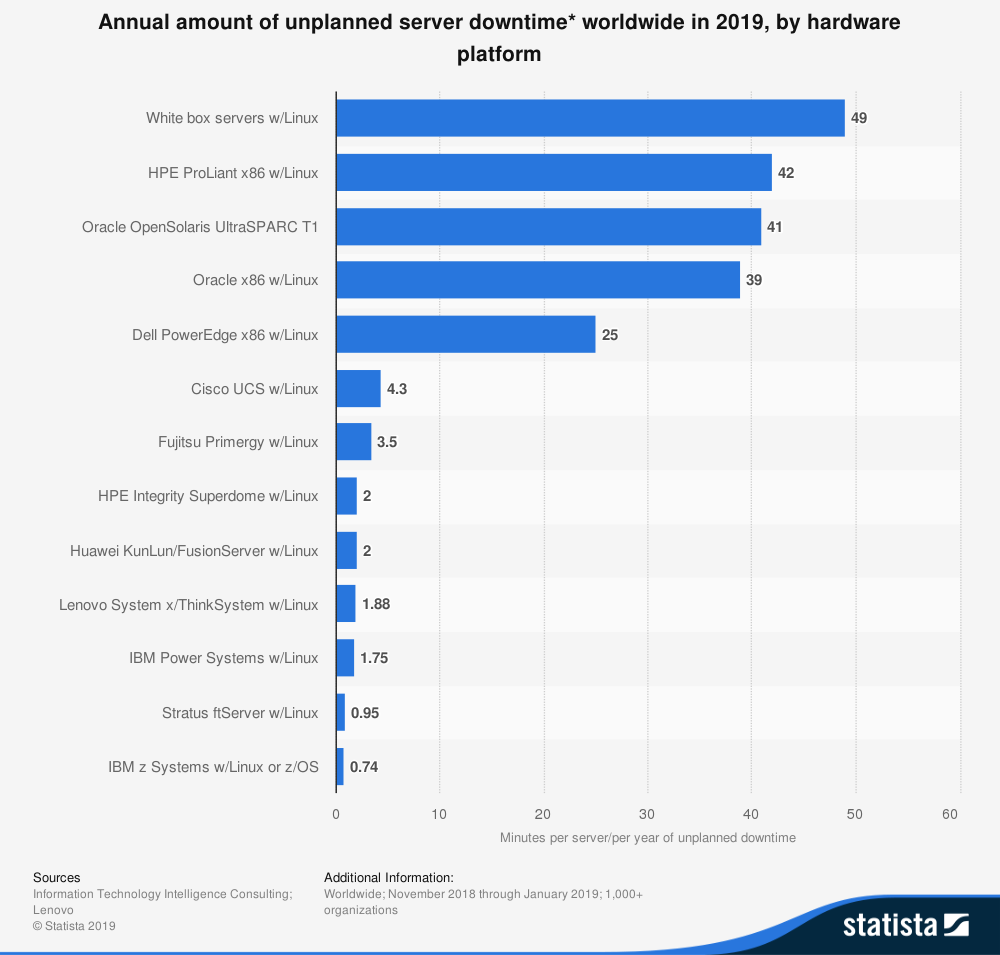
\includegraphics[width=\textwidth]{figures/statistic_id515285_unplanned-server-downtime-globally-2019-by-hardware-platform.png}
	\caption{Annual amount of unplanned server downtime worldwide in 2019, by hardeware platform}
	\label{fig:serverdowntime}
\end{figure}
Abbildung \ref{fig:serverdowntime} zeigt die ungeplannte Server Ausfallzeit in Minuten pro Server im Jahr 2019.
Wie zu sehen ist, schneidet der IBM z Systems w/Linux oder z/OS, das Mainframesystem der IBM, am besten ab.


Hinzu kommen spezielle Sicherheitsmechanismen und Skalierbarkeit.
All dies verbunden mit der durch (HIER SPECS EINFÜGEN) gewehrleisteten Performance, ermöglicht spezielle Use-Cases.
Unteranderem Massendatenverarbeitung, die dazugehörige Resourcenverwaltung und Breitband Kommunikation.
Das macht den Mainframe vor allem für Banken, das Gesundheitswesen, Versicherungen, Fluggesellschaften usw. attraktiv.
Zu diesen Unternehmen zählt auch die DATEV eG.
\cite{IBM.2014}

Die DATEV eG wurde am 14.02.1966 von 65 Steuerbevollmächtigten gegründet.
Sie verfolgten mit der Gründung das Ziel Buchführungsaufgaben mit Hilfe der EDV zu bewältigen.
Aufgrund hohen Mitgliederwachstums wurde hierfür 1969 in einen firmeneigenen IBM-Großrechner investiert.\cite{DATEVeG.2017}
Heute umfasst das Leistungsspektrum der DATEV eG unter anderen das Rechnungswesen, Personalwirtschaft, Consulting, IT-Sicherheit, Weiterbildung.
Ein nicht unbeträchtlicher Teil (PROZENTSATZ ?) der betriebswirtschaftlichen Anwendungen laufen bis heute auf einem IBM Großrechner.
So werden pro Tag circa 150.000 Batch Jobs und circa 90 Millionen CICS-Transaktionen verarbeitet.
Hierfür stehen dem System 114.000 MIPS an CPU-Kapazität zur Verfügung.
Diese Last wird von circa 14.000 aktiven Modulen erzeugt.
Wie in der Abbildung \ref{fig:Programmiersprachen} zu sehen ist, ist COBOL mit XXX Prozent die am häufigsten verwendete Programmiersprache am Großrechner bei der DATEV eG.
Durch diese Module werden unteranderem im Monat circa 13 Millionen Lohnabrechnungen erstellt und circa 1 Millionen Umsatzsteuer-Voranmeldungen durchgeführt.

Die Risiken die sich für die DATEV eG durch die Nutzung eines IBM Großrechners ergeben, werden im Folgenden dargestellt.\\
Zunächst ist zu nennen, dass die Verfügbarkeit von Skills im Mainframebereich immer schlechter wird.
Die aktuellen Wissenträger fallen durch ihr Alter langsam aus.
Durch die geringe Beliebtheit und wenig Präsenz an Universitäten und Hochschulen sind junge Nachfolger nur schwer zu finden.
So ist zum Beispiel die Programmiersprache auf den TIOBE Index Platz 28.\footnote{\cite{TIOBESoftwareBV.25.11.2019}}
Zum anderen gibt es in Deutschland nur XXX Universitäten und Hochschulen die einen Studiengang mit Schwerpunkt Mainframe anbieten.\cite{fehlt noch}

Als nächstes ist die Herstellerabhängigkeit von IBM zu erwähnen.
Die DATEV eG ist nicht nur in der Wahl eines Betriebssystems eingeschränkt, sondern auch einem Datenbanksystem oder einer Messaging Lösung.
Außerdem hat die IBM eine Quasi-Monopolstellung\cite{fehlt noch} im Mainframebereich, so ist die DATEV eG auch in ihrer Preisverhandlungspolitik eingeschränkt.
Hinzu kommt die Abhängigkeit von der IBM Mainframe Strategie, also ob die IBM selbst noch weitere Resourcen in ihren Großrechnerbereich investiert.
Dies wird durch eine sinkende Kundenzahl am Markt verstärkt.\footnote{weltweite installierte MIPS-Zahl sei laut IBM steigend}

Zuletzt ist der Modernisierungsbedarf beim Entwicklungsprozess zu nennen.





So gewinnen bei der DATEV eG PaaS (Plattform as a Service) Ansätze immer mehr an Bedeutung.
Ein Vorteil dabei ist die unkomplizierte, automatisierte Provisionierung von Laufzeitumgebungen.
Dadurch wird die Entwicklungsgeschwindigkeit erhöht und die Bereitstellung von isolierten Testumgebungen vereinfacht.
Außerdem können während eines laufenden Entwicklungsprozesses Komponenten, wie zum Beispiel ein Datenbanksystem, hinzugefügt oder ausgetauscht werden.
Bei der DATEV eG kommen diese Ansätze jedoch hauptsächlich bei Neuentwicklungen außerhalb des Mainframeumfelds zum Einsatz.




Was ist der Mainframe\\
Geschichte\\
kurzer technischer Einblick Mainframe und Vorteile und (Bedeutung bei Datev) \\
wieso er bei Datev eingesetzt wird \\
 Moma \\
 Problemstellung \\
 Wieso Rechnungsschreibung als Beispiel? \\